\begin{document}
\chapter{Procesarea de imagini pe dispozitive mobile}
	Dispozitivele mobile au avut o evolutie constanta pe parcursul timpului. In ziua de astazi multe dintre aceste dispozitive mobile ating perfomante mult mai ridicate decat ale unor laptopuri cu o vechime de 10 ani. 
	Desi dispozitivele mobile sunt perfecte pentru realizarea unor activitati de zi cu zi si sunt capabile sa faca fata unor aplicatii costisitoare din punctul de vedere al complexitatii, forta lor de computatie este relativa slaba, in comparatie cu cea a calculatoarelor si a laptopurilor. Dispozitivele mobile nu profita de aceeasi cantitatea de memorie CPU si GPU de care profita calculatoarele si laptopurile, rezultand intr-o peroada de timp prelungita necesara pentru finalizarea antrenarii unui model de retele neuronale cu un numar mare de filtre, straturi si operatii, cum ar fi augmentarea datelor.
	
	\section{Istoria dispozitvelor mobile}
	Ideea telefoanelor fara fir a aparut inca din perioada primului razboi mondial, cand armata germana testa comunicarea independenta de fir in interioriul trenurilor militare. Dezvoltarea acestor dispozitive de comunicare a luat amploare foarte repede. In jurul anului 1940, in perioada celui de al doilea razboi mondial, emitatoarele radio portabile jucau un rol crucial in comunicarea armatei.
	Tehnologia de comunicare prin emitatoare radio folosita de armata, a inspirat mai departe compania de cercetare stiintifca Bell Labs in crearea dispozitivelor dependente de masina, in anul 1946. Prin intermediul acestor dispozitive devenea posibila comunicarea telefonica din interiorul masinilor (vezi Fig. \ref{fig:tanti-telefon}).
	
	\begin{figure}[H]
		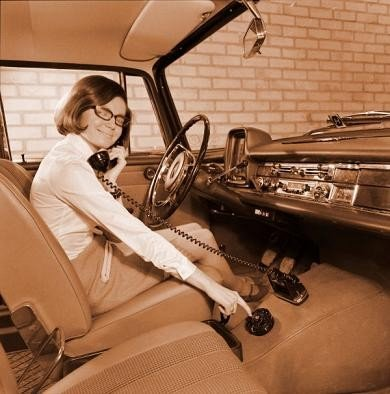
\includegraphics[width=10cm]{tanti-telefon}  
		\caption{\label{fig:tanti-telefon} Telefonul de masina creat de Bell Labs
			\protect
			\footnotemark}
	\end{figure}
	
	\footnotetext{http://www.realclear.com/offbeat/2016/02/03/\char`_did\char`_you\char`_know\char`_the\char`_first\char`_cell\char`_phone\char`_\\
		call\char`_was\char`_made\char`_out\char`_of\char`_spite\char`_12786.htm}
	
	La scurt timp dupa inovatia adusa de catre Bell Labs, AT\char`&T, compania americana specializata in telecomunicatii, va avea sa ofere servicii de telefonie mobila si canale de comunicare pe zone restranse. Dispozitivul oferit de catre AT\char`&T era asemanator un transmitator radio. Era necesara apasarea unui buton pentru a putea transmite un mesaj vocal, iar pentru a asculta interlocutorul, era necesara eliberarea butonului. Pentru a putea utiliza serviciile oferite de AT\char`&T in masina, era nevoie de atasarea unui echipament care cantarea aproximativ 36 de kg.
	In 1949, serviciul telefonic sustinut de AT\char`&T gazduia in jur de  5,000 de utilizatori, care realizau saptamanal aproximativ 30,000 de apeluri telefonice. Toate aceste apeluri telefonice erau gestionate manual de catre operatori ai companiei AT\char`&T. 
	
	Un serviciu asemanator celui oferit de AT\char`&T, a fost creat in Regatul Unit si se numea Post Office Radiophone Service. Diferenta facuta de acest serviciu telefonic a fost modul in care erau gestionate apeluri telefonice. Desi erau gestionate in continuare de un operator, un apel telefonic putea fi realizat intre oricare doi participanti din intregul Regat Unit. 
	
	Serviciul a fost creat in Manchester in 1959, adus in Londra in 1965, dupa care a fost distribuit in 1972 celorlalte orase mari din Anglia.
	In anul 1983 va avea sa apara primele telefoane mobile ce puteau fi tinute in mana. Primul producator de telefoane mobile a fost Motorola iar primul model a fost Motorola DynaTAC 8000x (vezi Fig.\ref{fig:dynatac}). Pretul sau crestea pana la 4000 de dolari, fiind un dispozitiv voluminos is greu (cantarind in jur de 4 kg)  avand o baterie capabila de a sustine 30 de minute de convorbire. In ciuda dimenisiunii mari a acestuia, era considerat cea mai buna varianta din punctul de vedere al portabilitatii datorita faptului ca va avea sa puna capat dependetei cablurilor telefonice pentru a purta o convorbire.
	
	\vfill
	
	\begin{figure}[H]
		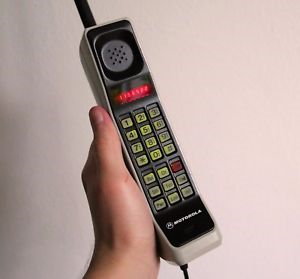
\includegraphics[width=8cm]{dynatac}  
		\caption{\label{fig:dynatac} Motorola DynaTAC 8000x
			\protect
			\footnotemark}
	\end{figure}
	
	\footnotetext{www.ebay.it}
	
	\vfill

	
	In anii 1990 au inceput sa aparata telefoane mobile apartinand generatiei a doua de dispozitive mobile. Acestea utilizau transmisie digitala, tehnologie ce aducea un plus de securitate si viteza peste transmisia analog. Odata cu aceasta generatie de dispozitive mobile, apar si SMS-urile (Short Message Service), prima utilizare fiind in 1993.
	In 1993, desi o teorie controversata, apare primul smartphone. IBM lanseaza modelul Simon. Acesta dispunea de: ceas, calendar, agenda telefonica, notite, casuta de email, auto-completare si touchscreen. (vezi Fig. \ref{fig:simon})
	
	
	
		\begin{figure}[H]
		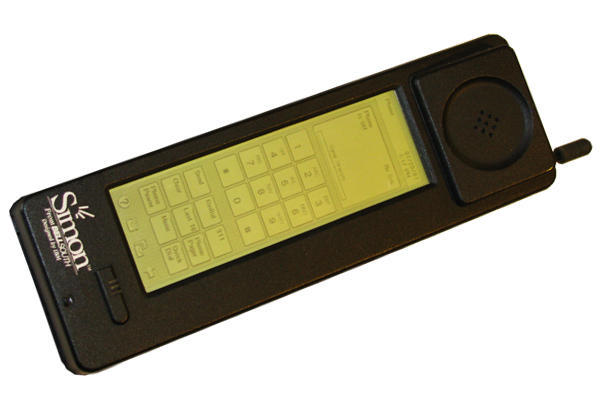
\includegraphics[width=8cm]{simon}  
		\caption{\label{fig:simon} Modelul de celular IBM Simon
			\protect
			\footnotemark}
	\end{figure}
	
	\footnotetext{shttps://www.androidauthority.com/ibm-simon-birthday-134255/}
	
	Dupa aparitia modelului Simon, creat de IBM, dispozitivele mobile vor avea sa urmeze un progres remarcabil in termen de functionalitate, stil si cel mai important, forta de computatie. 
	Telefoanele mobile au reusit sa introduca in buzunarul oamenilor forta de procesare, de la utilizarea unui simplu serviciu de email sau calendar, pana la utilizarea aplicatiilor ce dispun de inteligenta artificiala. \cite{history_cellphones}
	\newline
	
	\section{Sistemul de operare Android}
	
	Android este un sistem de operare Open Source dezvoltat si intretinut de catre compania Google. Google a cumparat in anul 2005 compania Android Inc., o companie ce se ocupa cu sisteme de operare pentru camere foto digitale si telfoane mobile, cu scopul intrarii pe piata dispozitivelor mobile. Dupa 2 ani de la cumpararea companiei, Google lanseaza sistemul de operare pe piata. 
	
	In momentul de fata, 85\% din totalitatea utilizatorilor dispozitivelor mobile smartphone, utlizeaza sistemul de operare Android. 
	
	Ceea ce face sistemul de operare Android, un punct de interes in viziunea invatarii automate, este arhitectura sa. Android are la baza o versiune a nucleului Linux, sistem de operare care face parte din familia UNIX. Sistemul de operare poate rula pe arhitecturi ARM. 
	
	Incepand din anul 2012, dispozitivele mobile Android sunt dezvoltate utliziand procesoare Intel iar mai tarziu se vor stabili pe arhitecturi de 64-bit, ARM64. 
	Forta pe care procesoarele dispozitivelor mobile o aduc, impreuna cu sistemul de operare Android, ne permit utilizarea multor tehnici de invatare automata chiar pe sistemul telefonului. 
	
	Desi placa de baza a dispozitivelor mobile permite rularea unor computatii complexe si utilizarea procesurilor si a firelor de executii, acestea permit de altfel utilizarea placii grafice (GPU), in scopul realizarii unor computatii intense distribuite.
	
	\subsection{Android System Developer Kit}
	
	Android System Developer Kit, sau Android SDK, este interfata expusa de Google, in scopul dezvoltarii de aplicatii si widgeturi pentru dispozitivele mobile Android, aparuta in 2008. Android SDK este un tool ce face  functionalitatile de baza ale telefonului mobil (cum ar fi camera, miscrofonul sau giroscopul) usor de utilizat, ofera biblioteci programabile, conditii de compilare, depanare si emulare a modelelor de dispozitive Android. 
	Sistemul de operare poate fi impartit in 5 componente:
	\begin{itemize}
		\item Aplications. Acestea sunt produsele finale la care au acces utilizatorii.
		
		
		\item Application Framework. Application Framework este baza programabila care usureaza utilizarea unor functionalitati precum: camera video sau foto, activitati, servicii de messaging, etc.
		
		\item Libraries. Penru a usura utilizarea bazelor de date, Secure Socket Layer, OpenGL, etc., au fost aduse la indemana programatorilor, biblioteci specializate in utilizarea acestor tehnologii.
		
		\item Android Runtime. Aplicatiile au nevoie de o masina virtuala pentru a rula. Android Runtime contine toate rutinele necesare pentru a compila si a rula o aplicatie.
		
		\item Linux Kernel. Pentru a accesa componentele hardware ale telefonului, sistemul de operare foloseste interefete numite "drivers". Acestea sunt rutine ce opereaza low-level cu placa de baza.
	\end{itemize}
	
	\vfill
	
	Pe parcursul dezvoltarii proiectului Android, acesta a trecut prin diferite versiuni, fiecare aducand o extensie in materie de functionalitati si imbunatatiri soft sistemului de operare. Desi proiectul era orientat spre progres, dezvoltarea s-a facut tinand cont de compatibilitatea anterioara. Astfel, versiunile noi ale sistemului de operare, pot rula aplicatii cu o vechime mai mare decat acestea.
	
	Prima versiune de Android a fost Astro 1.0. Aceasta rula pe modelul HTC Dream si detinea multe dintre aplicatiile care sunt inca utilizate in ziua de astazi. Printre aceste aplicatii se numara Android Market, Gmail, Google Maps etc.
	La aprope doi ani dupa aparitia versiunii Astro, apare versiunea 1.5 Cupcake. Aceasta rula pe un nucleu Linux 2.6, si a adus multe avantaje utilizatorilor si programatorilor. Aceasta versiune a introdus widgeturi, animatii si alte functionalitati la nivelul dispozitivelor cu Bluetooth.
	\newline
	
	Pe parcursul dezvoltarii, fiecare versiune aparuta a adus o imbunatatire in materie de funtionalitate sau interfata vizuala, insa un punct critic in dezvoltarea sistemului de operare si unul memorabil pentru invatarea automata, a fost versiunea 4.0, Ice Cream Sandwich. Aceasta versiunea a fost lansata in anul 2011 si este bazata pe un nucleu Linux, versiunea 3.0. Pe langa imbunatatirile aduse interfatei vizuale si flexibilitatii de configurare, versiunea Ice Cream Sandwich introduce utilizarea algoritmilor inteligenti de detectare a fetei si posibilitatea de a debloca telefonul utilizand recunoastere faciala. 	
	Acest punct marcheaza posibilitatea utilizarii algoritmilor de invatare automata pe dispozitivele mobile, fiind un imbold spre avansarea invatarii automate pe acest plan. Dezvoltarea proiectului a tinut cont din acest moment, de necesitatea utilizarea algoritmilor inteligenti pe dispozitive mobile, astfel s-a pus accent pe accelerarea hardware si minimalizarea costului sistemelor inteligente. Avansarea componentelor hardware nu constituie intregul motiv pentru care utilizarea algoritmilor inteligenti a devenit posibila, ci si simplificarea si optimizarea acestora pentru a fi utilizati in parametri optimi de rulare.
	\newline
	
	Desi exista alternative pentru dezvoltarea de aplicatii pe dispozitive Android, interfata oferita de Google este cea mai populara ca si numar de utilizatori. Un aspect important al acestei interfete, este flexibilitatea pe care o ofera, in materie de limbaje de programare. Aplicatiile Android pot fi dezvoltate pe baza Android SDK, utilizand limbajele de programare Java, C++ si Kotlin. \cite{android}	
	Android SDK expune modalitati de a procesa imaginile preluate din camera video a dispozitivului. Aceste modalitati, impreuna cu bilblioteci specializate in computatii distribuite utilizand forta GPU, ne permite utilizarea unor algoritm de invatare automata. 
	
	Android introduce in versiunea API 21 , o versiune noua a interfetei programabile ce gestioneaza camera video a dispozitivului mobil, Camera 2 API. Aceasta interfata acopera utilizarea camerei, de la permisiune pana la selectarea unei camere dintr-o lista de dispozitive disponibile si procesarea in mod continuu a imaginilor captate.
	
	
\end{document}